\documentclass{article}
\usepackage{tikz}
\usepgfmodule{nonlineartransformations}
\usetikzlibrary{shapes}
\usetikzlibrary{patterns}
\newcommand{\mytypeout}[1]{\relax}
\makeatletter
% from https://tex.stackexchange.com/q/56353/121799
\newcommand{\gettikzxy}[3]{%
  \tikz@scan@one@point\pgfutil@firstofone#1\relax
  \global\edef#2{\the\pgf@x}%
  \global\edef#3{\the\pgf@y}%
}
% from the manual section 103.4.2
% \pgf@x will contain the \xout{radius} angle
% \pgf@y will contain the distance \pgfmathsincos@{\pgf@sys@tonumber\pgf@x}%
% pgfmathresultx is now the cosine of \xout{radius} radius and 
% pgfmathresulty is the sine of radius 
% \pgf@x=\pgfmathresultx\pgf@y% 
% \pgf@y=\pgfmathresulty\pgf@y%
% what the thing in the pgf manually is probably doing it to express the x coordinate in pt
% then take the cos and sin of x/pt (i.e. if x=50pt then it will return cos(50))
% and multiply the outcome by a the y coordinate
% (x_new,y_new) = (y_old cos(x_old/pt), y_old sin(x_old/pt))
% now comes a slightly modified version
\def\marmotransformation{% modified version of the manual 103.4.2 Installing Nonlinear Transformation
\mytypeout{before:\space\the\pgf@x\space\the\pgf@y\space\xC\space\yC}%
\advance\pgf@x by -\xC% relative
\advance\pgf@y by -\yC% coorinates
\edef\relX{\the\pgf@x}%
\edef\relY{\the\pgf@y}% Yes, there is a more elegant solution based on \pgfpointadd
\mytypeout{xrel=\relX\space yrel=\relY}%
\pgfmathsetmacro{\relNx}{\xN-\xC}%
\pgfmathsetmacro{\relNy}{\yN-\yC}%
\pgfmathsetmacro{\angleN}{atan2(\relNy,\relNx)}%
\pgfmathsetmacro{\LeN}{veclen(\relNx,\relNy)}%
\mytypeout{relNx=\relNx,\space relNy=\relNy,\space LeN=\LeN,\space angleN=\angleN}%
\pgfmathsetmacro{\myp}{(\relX*\relNx+\relY*\relNy)/(\LeN*28.3465)}
\pgfmathsetmacro{\myo}{(((\relY*\relNx-\relX*\relNy))/(\myp*\LeN*(28.3465*pi/180)))+\angleN)}
\mytypeout{new\space p=\myp,\space o=\myo}
\pgfpointadd{\pgfqpoint{\xC}{\yC}}{\pgfpointpolarxy{\myo}{\myp}}
\mytypeout{after:\space\the\pgf@x\space\the\pgf@y}%
} % I have no idea why the factor 5 is needed
% I'm using https://tex.stackexchange.com/a/167109/121799
\begin{document}
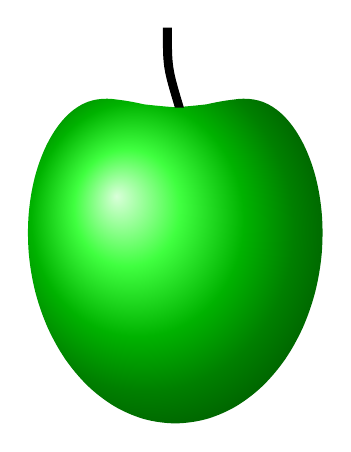
\begin{tikzpicture}
\coordinate (C) at (0,3) {};
\gettikzxy{(C)}{\xC}{\yC}
\coordinate (N) at (0,0) {};
\gettikzxy{(N)}{\xN}{\yN}
\begin{scope}[transform shape nonlinear=true]
\pgftransformnonlinear{\marmotransformation} 
\shade[shading=ball, ball color=green, opacity=1] (0,0) circle (2);
\end{scope}
\draw[smooth,fill=black](-0.15,3) .. controls (-0.15,2.5) .. (0,2) to 
(0.1,2) .. controls (-0.05,2.5) .. (-0.05,3) --cycle;
\end{tikzpicture}\hspace*{1cm}%
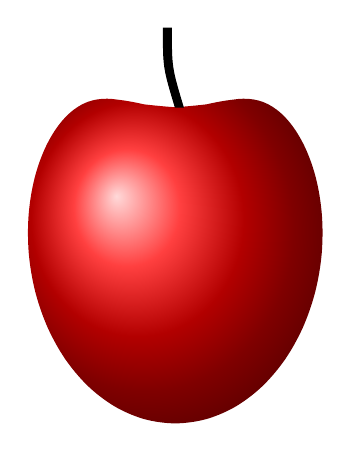
\begin{tikzpicture}
\coordinate (C) at (0,3) {};
\gettikzxy{(C)}{\xC}{\yC}
\coordinate (N) at (0,0) {};
\gettikzxy{(N)}{\xN}{\yN}
\begin{scope}[transform shape nonlinear=true]
\pgftransformnonlinear{\marmotransformation} 
\shade[shading=ball, ball color=red, opacity=1] (0,0) circle (2);
\end{scope}
\draw[smooth,fill=black](-0.15,3) .. controls (-0.15,2.5) .. (0,2) to 
(0.1,2) .. controls (-0.05,2.5) .. (-0.05,3) --cycle;
\end{tikzpicture}\hspace*{1cm}%
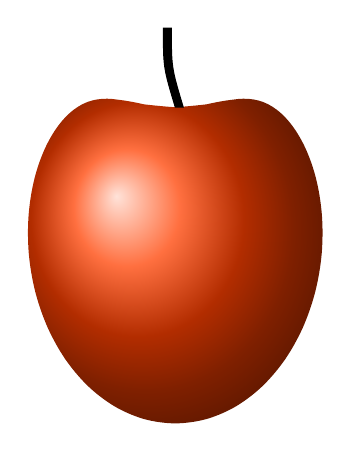
\begin{tikzpicture}
\coordinate (C) at (0,3) {};
\gettikzxy{(C)}{\xC}{\yC}
\coordinate (N) at (0,0) {};
\gettikzxy{(N)}{\xN}{\yN}
\begin{scope}[transform shape nonlinear=true]
\pgftransformnonlinear{\marmotransformation} 
\shade[shading=ball, ball color=red!50!orange, opacity=1] (0,0) circle (2);
\end{scope}
\draw[smooth,fill=black](-0.15,3) .. controls (-0.15,2.5) .. (0,2) to 
(0.1,2) .. controls (-0.05,2.5) .. (-0.05,3) --cycle;
\end{tikzpicture}
\end{document}
